% Generated by my modifications to the default Pandoc beamer template.
% Karl Browman has a tutorial about how to make Beamer sane:
% http://kbroman.wordpress.com/2013/10/07/better-looking-latexbeamer-slides/

% 12pt by default; handout if the handout template variable is defined
%\documentclass[12pt,handout,ignorenonframetext,]{beamer}
\documentclass[12pt,handout]{beamer}
\usetheme{metropolis}

\providecommand{\tightlist}{%
  \setlength{\itemsep}{0pt}\setlength{\parskip}{0pt}}

\usepackage{pgfpages}
\pgfpagesuselayout{2 on 1}

% theme, colortheme, and fonttheme with sensible defaults
%%\usetheme{metropolis}
%%%\usecolortheme{dove}
%%
% if it is a handout show the notes text; otherwise don't
\setbeameroption{show notes}
\setbeamertemplate{note page}[plain]

% Don't show things we don't want to see
\beamertemplatenavigationsymbolsempty
\hypersetup{pdfpagemode=UseNone} % don't show bookmarks on initial view

% Slide number in lower right
\definecolor{gray}{RGB}{155,155,155}
\setbeamertemplate{footline}{%
    \raisebox{5pt}{\makebox[\paperwidth]{\hfill\makebox[20pt]{\color{gray}
          \scriptsize\insertframenumber}}}\hspace*{5pt}}

% Space between paragraphs on notes page
\addtobeamertemplate{note page}{\setlength{\parskip}{12pt}}

% Color and shape of bullets
% \setbeamercolor{item}{fg=gray} 
% \setbeamercolor{subitem}{fg=gray}
% \setbeamercolor{itemize/enumerate subbody}{fg=gray}
\setbeamertemplate{itemize item}{{\textendash}}
\setbeamertemplate{itemize subitem}{{\textendash}}
\setbeamerfont{itemize/enumerate subbody}{size=\footnotesize}
\setbeamerfont{itemize/enumerate subitem}{size=\footnotesize}

\usepackage{amssymb,amsmath}
\usepackage{ifxetex,ifluatex}
\usepackage{fixltx2e} % provides \textsubscript
\ifxetex
  \usepackage{fontspec,xltxtra,xunicode}
  \defaultfontfeatures{Mapping=tex-text,Scale=MatchLowercase}
\else
  \ifluatex
    \usepackage{fontspec}
    \defaultfontfeatures{Mapping=tex-text,Scale=MatchLowercase}
  \else
    \usepackage[utf8]{inputenc}
  \fi
\fi
\usepackage{graphicx}
% Redefine \includegraphics so that, unless explicit options are
% given, the image width will not exceed the width of the page.
% Images get their normal width if they fit onto the page, but
% are scaled down if they would overflow the margins.
\makeatletter
\makeatother
\let\Oldincludegraphics\includegraphics
\renewcommand{\includegraphics}[2][]{\Oldincludegraphics[width=\textwidth,height=0.7\textheight,keepaspectratio]{#2}}

% Comment these out if you don't want a slide with just the
% part/section/subsection/subsubsection title:
%\AtBeginPart{
%  \let\insertpartnumber\relax
%  \let\partname\relax
%  \frame{\partpage}
%}
%\AtBeginSection{
%  \let\insertsectionnumber\relax
%  \let\sectionname\relax
%  \frame{\sectionpage}
%}
%\AtBeginSubsection{
%  \let\insertsubsectionnumber\relax
%  \let\subsectionname\relax
%  \frame{\subsectionpage}
%}

\setlength{\parindent}{0pt}
\setlength{\parskip}{6pt plus 2pt minus 1pt}
\setlength{\emergencystretch}{3em}  % prevent overfull lines
\setcounter{secnumdepth}{0}

\begin{document}

\begin{frame}{Continuum Mechanics}
\protect\hypertarget{continuum-mechanics}{}
Lecture 2 - Tensor Algebra

Dr.~Nicholas Smith

Wichita State University, Department of Aerospace Engineering

August 20, 2020
\end{frame}

\begin{frame}{schedule}
\protect\hypertarget{schedule}{}
\begin{itemize}
\tightlist
\item
  20 Aug - Tensor Algebra
\item
  25 Aug - Tensor Calculus, HW1 Due
\item
  27 Aug - Material Derivative
\item
  1 Sep - Conservation and Compatibility, HW2 Due
\end{itemize}
\end{frame}

\begin{frame}{outline}
\protect\hypertarget{outline}{}
\begin{itemize}
\tightlist
\item
  symmetry
\item
  transformation
\item
  examples
\item
  principal values
\item
  invariants
\item
  principal directions
\item
  examples
\end{itemize}
\end{frame}

\begin{frame}{symmetry}
\protect\hypertarget{symmetry}{}
\begin{itemize}
\tightlist
\item
  Symmetry can be a very powerful tool
\item
  Here we define some useful forms of symmetry in index notation
\item
  Symmetric

  \begin{itemize}
  \tightlist
  \item
    \(a_{ij...z} = a_{z...ji}\)
  \item
    \(a_{ij...m...n...z} = a_{ij...n...m...z}\)
  \end{itemize}
\item
  Anti-symmetric (skew symmetric)

  \begin{itemize}
  \tightlist
  \item
    \(a_{ij...z} = -a_{z...ji}\)
  \item
    \(a_{ij...m...n...z} = -a_{ij...n...m...z}\)
  \end{itemize}
\end{itemize}
\end{frame}

\begin{frame}{symmetry}
\protect\hypertarget{symmetry-1}{}
\begin{itemize}
\item
  Useful identity

  \begin{itemize}
  \tightlist
  \item
    If \(a_{ij...m...n...k}\) is symmetric in \(mn\) and
    \(b_{pq...m...n...r}\) is antisymmetric in \(mn\), then the product
    is zero
    {[}a\_\{ij\ldots m\ldots n\ldots k\}b\_\{pq\ldots m\ldots n\ldots r\}
    = 0{]}
  \end{itemize}
\item
  We can also write any tensor as the sum of its symmetric and
  anti-symmetric parts {[}a\_\{ij\} = \frac{1}{2} (a\_\{ij\} +
  a\_\{ji\}) + \frac{1}{2} (a\_\{ij\} - a\_\{ji\}){]}
\item
  This textbook uses a special shortcut notation (S and A superscript)
  for the symmetric and anti-symmetric portions of a tensor
\end{itemize}
\end{frame}

\begin{frame}{linear transformation}
\protect\hypertarget{linear-transformation}{}
\begin{itemize}
\item
  Let us consider some transformation, \(\textbf{T}\), which transforms
  any vector into another vector
\item
  If we transform \(\textbf{Ta} = c\) and \(\textbf{Tb} = d\)
\item
  We call \(\textbf{T}\) a linear transformation (and a tensor) if {[}

  \begin{aligned}
    \textbf{T}(\textbf{a} + \textbf{b}) &= \textbf{Ta} + \textbf{Tb}\\
    \textbf{T}(\alpha \textbf{a}) = \alpha\textbf{Ta}
  \end{aligned}

  {]}
\item
  Where \(\alpha\) is any arbitrary scalar and \(\textbf{a}\),
  \(\textbf{b}\) are arbitrary vectors
\end{itemize}
\end{frame}

\begin{frame}{2d coordinate transformation}
\protect\hypertarget{d-coordinate-transformation}{}
\begin{figure}
\centering
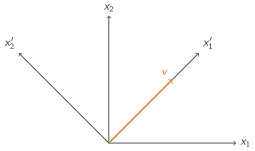
\includegraphics{../images/transform2d.svg}
\caption{2d coordinate transformation example with vector pointing from
(0,0) to (1,1)}
\end{figure}
\end{frame}

\begin{frame}{2d coordinate transformation}
\protect\hypertarget{d-coordinate-transformation-1}{}
\begin{itemize}
\tightlist
\item
  The vector, \(v\), remains fixed, but we transform our coordinate
  system
\item
  In the new coordinate system, the \(x_2^\prime\) portion of \(v\) is
  zero.
\item
  To transform the coordinate system, we first define some unit vectors.
\item
  \(\hat{e}_1\) is a unit vector in the direction of \(x_1\), while
  \(\hat{e}_1^\prime\) is a unit vector in the direction of
  \(x_1^\prime\)
\end{itemize}
\end{frame}

\begin{frame}{2d coordinate transformation}
\protect\hypertarget{d-coordinate-transformation-2}{}
\begin{figure}
\centering
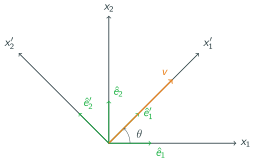
\includegraphics{../images/transform2d-unit.svg}
\caption{2d coordinate transformation from previous figure with unit
vectors drawn along the x and y axes}
\end{figure}
\end{frame}

\begin{frame}{2d coordinate transformation}
\protect\hypertarget{d-coordinate-transformation-3}{}
\begin{itemize}
\tightlist
\item
  For this example, let us assume \(v = \langle 2, 2 \rangle\) and
  \(\theta = 45^\circ\)
\item
  We can write the transformed unit vectors, \(\hat{e}_1^\prime\) and
  \(\hat{e}_2^\prime\) in terms of \(\hat{e}_1\), \(\hat{e}_2\) and the
  angle of rotation, \(\theta\). {[}

  \begin{aligned}
    \hat{e}_1^\prime &= \langle \hat{e}_1 \cos \theta , \hat{e}_2 \sin \theta\rangle\\
    \hat{e}_2^\prime &= \langle -\hat{e}_1 \sin \theta , \hat{e}_2 \cos \theta \rangle
  \end{aligned}

  {]}
\end{itemize}
\end{frame}

\begin{frame}{2d coordinate transformation}
\protect\hypertarget{d-coordinate-transformation-4}{}
\begin{itemize}
\tightlist
\item
  We can write the vector, \(v\), in terms of the unit vectors
  describing our axis system
\item
  \(v = v_1 \hat{e}_1 + v_2 \hat{e}_2\)
\item
  (note: \(\hat{e}_1=\langle 1, 0 \rangle\) and
  \(\hat{e}_2 = \langle 0,1 \rangle\))
\item
  \(v = \langle 2, 2 \rangle = 2 \langle 1, 0 \rangle + 2 \langle 0,1 \rangle\)
\end{itemize}
\end{frame}

\begin{frame}{2d coordinate transformation}
\protect\hypertarget{d-coordinate-transformation-5}{}
\begin{itemize}
\tightlist
\item
  When expressed in the transformed coordinate system, we refer to
  \(v^\prime\)
\item
  \(v^\prime = \langle v_1 \cos \theta + v_2 \sin \theta, -v_1 \sin \theta + v_2 \cos \theta \rangle\)
\item
  \(v^\prime = \langle 2\sqrt{2}, 0 \rangle\)
\item
  We can recover the original vector from the transformed coordinates:
\item
  \(v = v_1^\prime \hat{e}_1^\prime + v_2^\prime \hat{e}_2^\prime\)
\item
  (note:
  {[}\hat{e}\_1\^{}\prime=\langle \frac{\sqrt{2}}{2},\frac{\sqrt{2}}{2}
  \rangle{]} and {[}\hat{e}\_2\^{}\prime =
  \langle -\frac{\sqrt{2}}{2},\frac{\sqrt{2}}{2} \rangle{]}) {[}v =
  2\sqrt{2}\langle \frac{\sqrt{2}}{2},\frac{\sqrt{2}}{2} \rangle, 0
  \langle -\frac{\sqrt{2}}{2},\frac{\sqrt{2}}{2} \rangle = \langle 2, 2
  \rangle{]}
\end{itemize}
\end{frame}

\begin{frame}{coordinate transformation}
\protect\hypertarget{coordinate-transformation}{}
\begin{itemize}
\tightlist
\item
  Coordinate transformation can become much more complicated in three
  dimensions, and with higher-order tensors
\item
  We define \(Q_{ij}\) as the cosine of the angle between the
  \(x_i^\prime\) axis and the \(x_j\) axis.
\item
  This is also referred to as the ``direction cosine'' {[}Q\_\{ij\} =
  \cos (x\_i\^{}\prime, x\_j){]}
\item
  \emph{health warning} the direction cosine can also be defined
  inversely (\(Q_{ij} =\cos (x_i, x_j^\prime)\)), and the indexes are
  switched in the transformation law
\end{itemize}
\end{frame}

\begin{frame}{coordinate transformation}
\protect\hypertarget{coordinate-transformation-1}{}
\begin{itemize}
\tightlist
\item
  We can use this form on our 2D transformation example {[}

  \begin{aligned}
    Q_{ij} &= \cos (x_i^\prime, x_j)\ &= \begin{bmatrix}
    \cos (x_1^\prime, x_1) & \cos (x_1^\prime, x_2)\\
    \cos (x_2^\prime, x_1) & \cos (x_2^\prime, x_2)
    \end{bmatrix}\ &= \begin{bmatrix}
    \cos \theta & \cos (90-\theta)\\
    \cos (90+\theta) & \cos \theta
    \end{bmatrix} \ &= \begin{bmatrix}
    \cos \theta & \sin \theta \\
    -\sin \theta & \cos \theta
    \end{bmatrix}
  \end{aligned}

  {]}
\end{itemize}
\end{frame}

\begin{frame}{coordinate transformation}
\protect\hypertarget{coordinate-transformation-2}{}
\begin{itemize}
\tightlist
\item
  We can transform any-order tensor using \(Q_{ij}\)
\item
  Vectors (first-order tensors): \(v^\prime_i = Q_{ij}v_j\)
\item
  Matrices (second-order tensors):
  {[}\sigma\emph{\{mn\}\^{}\prime =Q}\{mi\}Q\_\{nj\}\sigma\_\{ij\}{]}
\item
  Fourth-order tensors: {[}C\_\{ijkl\}\^{}\prime =
  Q\_\{im\}Q\_\{jn\}Q\_\{ko\}Q\_\{lp\}C\_\{mnop\}{]}
\end{itemize}
\end{frame}

\begin{frame}{coordinate transformation}
\protect\hypertarget{coordinate-transformation-3}{}
\begin{itemize}
\tightlist
\item
  We can similarly use \(Q_{ij}\) to find tensors in the original
  coordinate system
\item
  Vectors (first-order tensors): \(v_i = Q_{ji}v_j^\prime\)
\item
  Matrices (second-order tensors):
  \(\sigma_{mn} =Q_{im}Q_{jn}\sigma_{ij}^\prime\)
\item
  Fourth-order tensors:
  \(C_{ijkl} = Q_{mi}Q_{nj}Q_{ok}Q_{pl}C_{mnop}^\prime\)
\end{itemize}
\end{frame}

\begin{frame}{coordinate transformation}
\protect\hypertarget{coordinate-transformation-4}{}
\begin{itemize}
\tightlist
\item
  We can derive some interesting properties of the transformation
  tensor, \(Q_{ij}\)
\item
  We know that \(v_i = Q_{ji}v_j^\prime\) and that
  \(v^\prime_i = Q_{ij}v_j\)
\item
  If we substitute (changing the appropriate indexes) we find: {[}v\_i =
  Q\_\{ji\}Q\_\{jk\}v\_k{]}
\item
  We can now use the Kronecker Delta to substitute
  \(v_i = \delta_{ik}v_k\) which gives {[}\delta\emph{\{ik\}v\_k =
  Q}\{ji\}Q\_\{jk\}v\_k{]}
\end{itemize}
\end{frame}

\begin{frame}{example}
\protect\hypertarget{example}{}
\begin{figure}
\centering
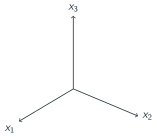
\includegraphics{../images/transform3d-1.svg}
\caption{3d coordinate system to start general transformation example}
\end{figure}

\begin{itemize}
\tightlist
\item
  Find \(Q_{ij}^1\) for rotation of \(60^\circ\) about \(x_2\)
\item
  Find \(Q_{ij}^2\) for rotation of \(30^\circ\) about \(x_3^\prime\)
\item
  Find \({e}_i^{\prime\prime}\) after both rotations
\end{itemize}
\end{frame}

\begin{frame}{example}
\protect\hypertarget{example-1}{}
\begin{figure}
\centering
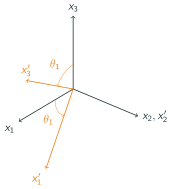
\includegraphics{../images/transform3d-2.svg}
\caption{3d illustration of first transformation}
\end{figure}
\end{frame}

\begin{frame}{example}
\protect\hypertarget{example-2}{}
\begin{figure}
\centering
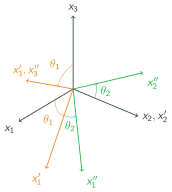
\includegraphics{../images/transform3d-3.svg}
\caption{3d illustration of second transformation (about the axes of the
first)}
\end{figure}
\end{frame}

\begin{frame}{example}
\protect\hypertarget{example-3}{}
\begin{itemize}
\tightlist
\item
  \(Q_{ij}^1 = \cos (x_i^\prime,x_j)\)
\item
  \(Q_{ij}^2 = \cos (x_i^{\prime\prime},x_j^\prime)\) {[}Q\_\{ij\}\^{}1
  =

  \begin{bmatrix}
    \cos 60 & \cos 90 & \cos 150\\
    \cos 90 & \cos 0 & \cos 90\\
    \cos 30 & \cos 90 & \cos 60
    \end{bmatrix}

  {]} {[}Q\_\{ij\}\^{}2 =

  \begin{bmatrix}
    \cos 30 & \cos 60 & \cos 90\\
    \cos 120 & \cos 30 & \cos 90\\
    \cos 90 & \cos 90 & \cos 0
  \end{bmatrix}

  {]}
\end{itemize}
\end{frame}

\begin{frame}{example}
\protect\hypertarget{example-4}{}
\begin{itemize}
\tightlist
\item
  We now use \(Q_{ij}\) to find \(\hat{e}_i^\prime\) and
  \(\hat{e}_i^{\prime \prime}\)
\item
  First, we need to write \(\hat{e}_i\) in a manner more consistent with
  index notation
\item
  We will indicate axis direction with a superscript,
  e.g.~\(\hat{e}_1 = e_i^1\)
\item
  \(e_i^\prime = Q^1_{ij} e_j\)
\item
  \(e_i^{\prime\prime} = Q^2_{ij} e_j^\prime\)
\end{itemize}
\end{frame}

\begin{frame}{example}
\protect\hypertarget{example-5}{}
\begin{itemize}
\tightlist
\item
  How do we find \(e_i^{\prime\prime}\) in terms of \(e_i\)?
\item
  \(e_i^{\prime\prime} = Q^2_{ij} Q^1_{jk} e_k\)
\end{itemize}
\end{frame}

\begin{frame}{principal values}
\protect\hypertarget{principal-values}{}
\begin{itemize}
\tightlist
\item
  In the 2D coordinate transformation example, we were able to eliminate
  one value from a vector using coordinate transformation
\item
  For second-order tensors, we desire to find the ``principal values''
  where all non-diagonal terms are zero
\item
  The direction determined by the unit vector, \(n_j\), is said to be
  the \emph{principal direction} or \emph{eigenvector} of the symmetric
  second-order tensor, \(a_{ij}\) if there exists a parameter,
  \(\lambda\), such that {[}a\_\{ij\} n\_j = \lambda n\_i{]}
\item
  Where \(\lambda\) is called the \emph{principal value} or
  \emph{eigenvalue} of the tensor
\end{itemize}
\end{frame}

\begin{frame}{principal values}
\protect\hypertarget{principal-values-1}{}
\begin{itemize}
\item
  We can re-write the equation {[}(a\_\{ij\} -
  \lambda \delta\_\{ij\})n\_j = 0{]}
\item
  This system of equations has a non-trivial solution if and only if
  \(\det [a_{ij} - \lambda \delta_{ij}] = 0\)
\item
  This equation is known as the characteristic equation, and we solve it
  to find the principal values of a tensor
\end{itemize}
\end{frame}

\begin{frame}{example}
\protect\hypertarget{example-6}{}
\begin{itemize}
\item
  Find the principal values of the tensor {[}A\_\{ij\} =

  \begin{bmatrix}
    1 & 2\\
    2 & 4
  \end{bmatrix}

  {]}
\item
  From the characteristic equation, we know that
  \(\det [A_{ij} - \lambda \delta_{ij}] = 0\), or {[}

  \begin{vmatrix}
    1-\lambda & 2\\
    2 & 4 - \lambda
  \end{vmatrix}

  = 0{]}
\end{itemize}
\end{frame}

\begin{frame}{example}
\protect\hypertarget{example-7}{}
\begin{itemize}
\item
  Calculating the determinant gives {[}(1-\lambda)(4-\lambda) - 4 = 0{]}
\item
  Multiplying out and simplifying, we find {[}\lambda\^{}2 - 5\lambda =
  \lambda(\lambda-5) = 0{]}
\item
  This has the solution \(\lambda = 0, 5\)
\end{itemize}
\end{frame}

\begin{frame}{invariants}
\protect\hypertarget{invariants}{}
\begin{itemize}
\tightlist
\item
  Every tensor has some invariants which do not change with coordinate
  transformation
\item
  These are known as \emph{fundamental invariants}
\item
  The characteristic equation for a tensor in 3D can be written in terms
  of the invariants {[}\det [ a_{ij} - \lambda \delta_{ij}] =
  -\lambda\^{}3 + I\_\alpha \lambda\^{}2 - II\_\alpha \lambda +
  III\_\alpha = 0{]}
\end{itemize}
\end{frame}

\begin{frame}{invariants}
\protect\hypertarget{invariants-1}{}
\begin{itemize}
\tightlist
\item
  The invariants can be found by the following equations {[}

  \begin{aligned}
    I_\alpha &= a_{ii}\\
    II_\alpha &= \frac{1}{2}(a_{ii} a_{jj} - a_{ij}a_{ij})\\
    III_\alpha &= \det [ a_{ij}]
  \end{aligned}

  {]}
\end{itemize}
\end{frame}

\begin{frame}{invariants}
\protect\hypertarget{invariants-2}{}
\begin{itemize}
\item
  In the principal direction, \(a_{ij}^\prime\) will be
  {[}a\_\{ij\}\^{}\prime =

  \begin{bmatrix}
    \lambda_1 & 0 & 0\\
    0 & \lambda_2 & 0\\
    0 & 0 & \lambda_3
  \end{bmatrix}

  {]}
\item
  Since invariants do not change with coordinate systems, we can also
  write the invariants as {[}

  \begin{aligned}
    I_\alpha &= \lambda_1 + \lambda_2 + \lambda_3\\
    II_\alpha &= \lambda_1\lambda_2 + \lambda_2 \lambda_3 + \lambda_3 \lambda_1\\
    III_\alpha &= \lambda_1 \lambda_2 \lambda_3
  \end{aligned}

  {]}
\end{itemize}
\end{frame}

\begin{frame}{principal directions}
\protect\hypertarget{principal-directions}{}
\begin{itemize}
\item
  We defined principal directions earlier {[}(a\_\{ij\} -
  \lambda \delta\_\{ij\})n\_j = 0{]}
\item
  \(\lambda\) are the principal values and \(n_j\) are the principal
  directions
\item
  For each eigenvalue there will be a principal direction
\item
  We find the principal direction by substituting the solution for
  \(\lambda\) back into this equation
\end{itemize}
\end{frame}

\begin{frame}{example}
\protect\hypertarget{example-8}{}
\begin{itemize}
\item
  Find the principal directions for the earlier principal values example
\item
  Recall \(\lambda = 0,5\), let us say \(\lambda_1 = 5\), we find
  \(n_j^{(1)}\) by {[}

  \begin{bmatrix}
    1-\lambda_1 & 2\\
    2 & 4-\lambda_1
  \end{bmatrix} \begin{Bmatrix}
    n_1 \ n_2
  \end{Bmatrix}

  = 0{]}
\item
  This gives {[}

  \begin{bmatrix}
    -4 & 2\\
    2 & -1
  \end{bmatrix} \begin{Bmatrix}
    n_1 \ n_2
  \end{Bmatrix}

  = 0{]}
\end{itemize}
\end{frame}

\begin{frame}{example}
\protect\hypertarget{example-9}{}
\begin{itemize}
\item
  We proceed to solve the equations using row-reduction, but we find {[}

  \begin{bmatrix}
    2 & -1\\
    0 & 0
  \end{bmatrix} \begin{Bmatrix}
    n_1 \ n_2
  \end{Bmatrix}

  = 0{]}
\item
  This means we cannot uniquely solve for \(n_j\)
\item
  We are only concerned with the direction, magnitude is not important
\item
  Choose \(n_2 = 1\), solve for \(n_1\)
\item
  \(n^{(1)} = \langle \frac{1}{2}, 1 \rangle\)
\end{itemize}
\end{frame}

\begin{frame}{example}
\protect\hypertarget{example-10}{}
\begin{itemize}
\item
  Similarly, for \(\lambda_2 =0\), we find {[}

  \begin{bmatrix}
    1 & 2\\
    2 & 4
  \end{bmatrix} \begin{Bmatrix}
    n_1 \ n_2
  \end{Bmatrix}

  = 0{]}
\item
  Which, after row-reduction, becomes {[}

  \begin{bmatrix}
    1 & 2\\
    0 & 0
  \end{bmatrix} \begin{Bmatrix}
    n_1 \ n_2
  \end{Bmatrix}

  = 0{]}
\item
  If we choose \(n_2 = 1\), we find \(n_1 = -2\)
\item
  This gives \(n^{(2)} = \langle -2, 1 \rangle\)
\end{itemize}
\end{frame}

\begin{frame}{example}
\protect\hypertarget{example-11}{}
\begin{itemize}
\tightlist
\item
  We can assemble a transformation matrix, \(Q_{ij}\), from the
  principal directions
\item
  First we need to normalize them to unit vectors
\item
  \(||n^{(1)}|| = \sqrt{\frac{5}{4}}\)
\item
  \(\hat{n}^{(1)} = \frac{2}{\sqrt{5}} \langle \frac{1}{2}, 1 \rangle = \langle \frac{1}{\sqrt{5}}, \frac{2}{\sqrt{5}} \rangle\)
\item
  \(||n^{(2)}|| = \sqrt{5}\)
\item
  \(\hat{n}^{(2)} = \langle \frac{-2}{\sqrt{5}}, \frac{1}{\sqrt{5}} \rangle\)
\end{itemize}
\end{frame}

\begin{frame}{example}
\protect\hypertarget{example-12}{}
\begin{itemize}
\item
  This gives {[}Q\_\{ij\} = \frac{1}{\sqrt{5}}

  \begin{bmatrix}
    1 & 2\\
    -2 & 1
  \end{bmatrix}

  {]}
\item
  And we find {[}A\_\{mn\}\^{}\prime = Q\_\{mi\}Q\_\{nj\}A\_\{ij\}{]}
  {[}A\_\{ij\}\^{}\prime =

  \begin{bmatrix}
    5 & 0 \\
    0 & 0
  \end{bmatrix}

  {]}
\end{itemize}
\end{frame}

\begin{frame}{example}
\protect\hypertarget{example-13}{}
\begin{itemize}
\tightlist
\item
  Find principal values, principal directions, and invariants for the
  tensor {[}c\_\{ij\} =

  \begin{bmatrix}
    8 & 0 & 0\\
    0 & 3 & 1\\
    0 & 1 & 3
  \end{bmatrix}

  {]}
\end{itemize}
\end{frame}

\begin{frame}{example}
\protect\hypertarget{example-14}{}
\begin{itemize}
\tightlist
\item
  Characteristic equation simplifies to
\item
  \(-\lambda^3 + 14\lambda^2 -56 \lambda + 64 = 0\)
\item
  Which has the solutions \(\lambda = 2, 4, 8\)
\end{itemize}
\end{frame}

\begin{frame}{example}
\protect\hypertarget{example-15}{}
\begin{itemize}
\tightlist
\item
  To find the principal direction for \(\lambda_1 = 8\) {[}

  \begin{bmatrix}
    8-8 & 0 & 0\\
    0 & 3-8 & 1\\
    0 & 1 & 3-8
  \end{bmatrix}\begin{Bmatrix}
    n_1 \ n_2 \ n_3
  \end{Bmatrix}

  = 0{]}
\end{itemize}
\end{frame}

\begin{frame}{example}
\protect\hypertarget{example-16}{}
\begin{itemize}
\item
  After row-reduction, we find {[}

  \begin{bmatrix}
    0 & 0 & 0\\
    0 & 0 & -24\\
    0 & 1 & -5
  \end{bmatrix}\begin{Bmatrix}
    n_1 \ n_2 \ n_3
  \end{Bmatrix}

  = 0{]}
\item
  This means that \(n_3 = 0\) and, as a result, \(n_2 = 0\).
\item
  \(n_1\) can be any value, we choose \(n_1 = 1\) to give a unit vector.
\item
  \(n^{(1)} = \langle 1, 0, 0 \rangle\)
\end{itemize}
\end{frame}

\begin{frame}{example}
\protect\hypertarget{example-17}{}
\begin{itemize}
\tightlist
\item
  To find the principal direction for \(\lambda_2 = 4\) {[}

  \begin{bmatrix}
    8-4 & 0 & 0\\
    0 & 3-4 & 1\\
    0 & 1 & 3-4
  \end{bmatrix}\begin{Bmatrix}
    n_1 \ n_2 \ n_3
  \end{Bmatrix}

  = 0{]}
\end{itemize}
\end{frame}

\begin{frame}{example}
\protect\hypertarget{example-18}{}
\begin{itemize}
\item
  After row-reduction, we find {[}

  \begin{bmatrix}
    4 & 0 & 0\\
    0 & -1 & 1\\
    0 & 0 & 0
  \end{bmatrix}\begin{Bmatrix}
    n_1 \ n_2 \ n_3
  \end{Bmatrix}

  = 0{]}
\item
  This means that \(n_1 = 0\)
\item
  We also know that \(n_2 = n_3\), so we choose \(n_2 = n_1 = 1\)
\item
  This gives \(n^{(2)} = \frac{1}{\sqrt{2}}\langle 0, 1, 1 \rangle\)
  after normalization
\end{itemize}
\end{frame}

\begin{frame}{example}
\protect\hypertarget{example-19}{}
\begin{itemize}
\tightlist
\item
  To find the principal direction for \(\lambda_3 = 2\) {[}

  \begin{bmatrix}
    8-2 & 0 & 0\\
    0 & 3-2 & 1\\
    0 & 1 & 3-2
  \end{bmatrix}\begin{Bmatrix}
    n_1 \ n_2 \ n_3
  \end{Bmatrix}

  = 0{]}
\end{itemize}
\end{frame}

\begin{frame}{example}
\protect\hypertarget{example-20}{}
\begin{itemize}
\item
  After row-reduction, we find {[}

  \begin{bmatrix}
    6 & 0 & 0\\
    0 & 1 & 1\\
    0 & 0 & 0
  \end{bmatrix}\begin{Bmatrix}
    n_1 \ n_2 \ n_3
  \end{Bmatrix}

  = 0{]}
\item
  This means that \(n_1 = 0\)
\item
  We also know that \(n_2 = -n_3\), so we choose \(n_2 = 1\) and
  \(n_1 = -1\)
\item
  This gives \(n^{(3)} = \frac{1}{\sqrt{2}}\langle 0, 1, -1 \rangle\)
  after normalization
\end{itemize}
\end{frame}

\begin{frame}{example}
\protect\hypertarget{example-21}{}
\begin{itemize}
\tightlist
\item
  In summary, for \(c_{ij}\) we have:
\item
  \(\lambda_1 = 8\) and \(n^{(1)} = \langle 1, 0, 0 \rangle\)
\item
  \(\lambda_2 = 4\) and
  \(n^{(2)} = \frac{1}{\sqrt{2}}\langle 0, 1, 1 \rangle\)
\item
  \(\lambda_3 = 2\) and
  \(n^{(3)} = \frac{1}{\sqrt{2}}\langle 0, 1, -1 \rangle\)
\item
  We can assemble \(n^{(i)}\) into a transformation tensor {[}Q\_\{ij\}
  = \frac{1}{\sqrt{2}}

  \begin{bmatrix}
    \sqrt{2} & 0 & 0\\
    0 & 1 & 1\\
    0 & 1 & -1
  \end{bmatrix}

  {]}
\end{itemize}
\end{frame}

\begin{frame}{example}
\protect\hypertarget{example-22}{}
\begin{itemize}
\tightlist
\item
  What is \(c_{ij}^\prime\)?
\item
  \(c_{ij}^\prime = Q_{im}Q_{jn}c_{mn}\) {[}c\_\{ij\}\^{}\prime =

  \begin{bmatrix}
    8 & 0 & 0 \\
    0 & 4 & 0 \\
    0 & 0 & 2
  \end{bmatrix}

  {]}
\end{itemize}
\end{frame}

\begin{frame}{example}
\protect\hypertarget{example-23}{}
\begin{itemize}
\item
  We can also find the invariants for {[}c\_\{ij\} =

  \begin{bmatrix}
    8 & 0 & 0\\
    0 & 3 & 1\\
    0 & 1 & 3
  \end{bmatrix}

  {]}
\item
  Recall: {[}

  \begin{aligned}
    I_\alpha &= a_{ii}\\
    II_\alpha &= \frac{1}{2}(a_{ii} a_{jj} - a_{ij}a_{ij})\\
    III_\alpha &= \det [ a_{ij}]
  \end{aligned}

  {]}
\end{itemize}
\end{frame}

\begin{frame}{example}
\protect\hypertarget{example-24}{}
\begin{itemize}
\tightlist
\item
  First invariant {[}I\_\alpha = a\_\{ii\} = 8 + 3 + 3 = 14{]}
\item
  Second invariant {[}II\_\alpha = \frac{1}{2}(a\_\{ii\} a\_\{jj\} -
  a\_\{ij\}a\_\{ij\}){]} {[}a\_\{ii\} a\_\{jj\} = 14 \times 14{]}
  {[}a\_\{ij\}a\_\{ij\} = a\_\{11\}a\_\{11\} + a\_\{12\}a\_\{12\} +
  a\_\{13\}a\_\{13\} + \ldots{} + a\_\{33\}a\_\{33\}{]} {[}II\_\alpha =
  \frac{1}{2}(196 - 84) = 56{]}
\end{itemize}
\end{frame}

\begin{frame}{example}
\protect\hypertarget{example-25}{}
\begin{itemize}
\tightlist
\item
  Third invariant {[}III\_\alpha = \det [ a_{ij}]{]} {[}III\_\alpha = 8
  \times (3 \times 3 - 1 \times 1) = 64{]}
\end{itemize}
\end{frame}

\end{document}
